\documentclass[10pt,a4paper]{article}

\usepackage[margin=0.75cm]{geometry}
\usepackage[utf8]{inputenc}

\usepackage{amsmath}
\usepackage{amssymb}
\usepackage{biblatex}
\usepackage{textcomp}
\usepackage{gensymb}
\usepackage{paracol}
\usepackage{parskip}
\usepackage{tikz}
\usepackage{titlesec}
\usepackage{verbatim}
\usepackage{xcolor}

\titleformat{\section}[block]{\Large\bfseries\filcenter\color{black}}{\thesection}{1em}{}
\titleformat{\subsection}[block]{\bfseries\filcenter\color{black}}{\thesubsection}{1em}{}

\setlength{\columnsep}{25pt}

\tikzset{
    rounded-box/.style = {draw=orange, fill=white, thin, rectangle, rounded corners, inner sep=5pt, inner ysep=10pt},
    rounded-box-title/.style = {fill=orange, text=white, font=\bfseries},
}

\addbibresource{references.bib}

\begin{document}
\title{Statistics}

\section{Descriptive Statistics}

\begin{paracol}{2}

\begin{center}
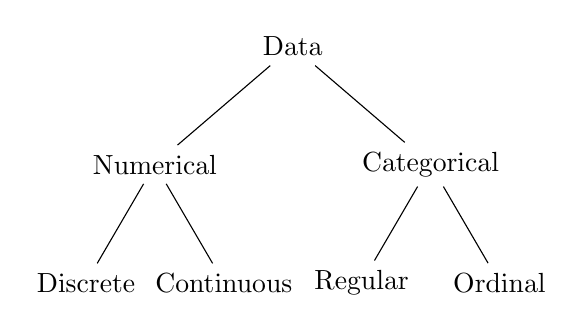
\begin{tikzpicture}[level distance=1.5cm,
  level 1/.style={sibling distance=3.5cm},
  level 2/.style={sibling distance=1.75cm}]
  \node {Data}
    child {node {Numerical}
      child {node {Discrete}}
      child {node {Continuous}}
    }
    child {node {Categorical}
      child {node {Regular}}
      child {node {Ordinal}}
    };
\end{tikzpicture}
\end{center}

\switchcolumn

Observational data come from observing the world as it is.

Experimental data are generated by designing an experiment to test the effect of some explanatory variable, e.g. giving a treatment to the treatment group while not giving it to the control group (/only pretending to treat them).

A summary \textbf{statistic} is a number summarising the data, e.g. the mean, median (middle value), mode (most common value), variance.

\end{paracol}

Imagine we take a sample of $n$ observations from a population and calculate a sample statistic. Now imagine we take another $n$ observations and another $n$ observations, etc., and each time we calculate the sample statistic. We can then plot the distribution of the sampling statistic - this is a \textbf{sampling distribution}. By the CLT, for a large number of successive random samples (big $n$), the distribution of sample means calculated for each sample will become approximately normally distributed.

If you take a lot of sample means from the same population, you may get a different result each time and perhaps none of the sample means would exactly equal the true population mean. Therefore, we need to specify a \textbf{margin of error} - a confidence interval. Point estimates vary from sample to sample, and we quantify this variability with what is called the standard error - the standard deviation of the sampling distribution:

\vspace{-20pt}

$$SE = \sqrt{\text{Var}(\bar{X}) = \sqrt{\frac{\sigma^2}{n}}}$$

\vspace{-10pt}

Confidence interval: point estimate $\pm z^* \times SE$, where $z^* \times SE$ is the margin of error.

\subsection{Connection with Probability Theory}

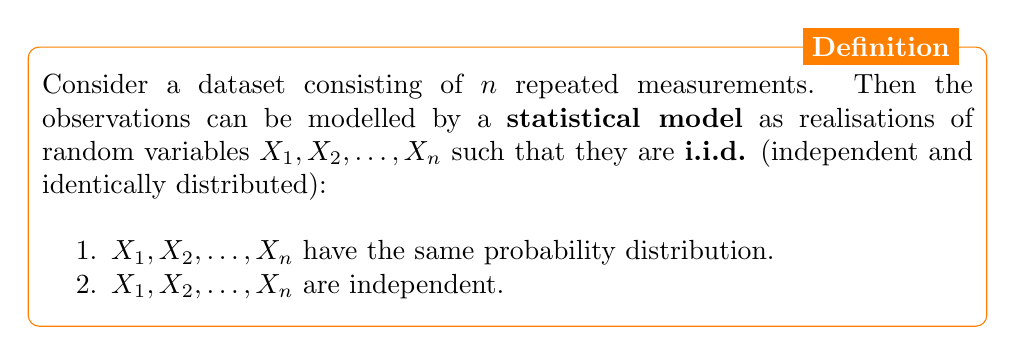
\begin{tikzpicture}
\node [rounded-box] (box){\begin{minipage}{0.975\textwidth}
    Consider a dataset consisting of $n$ repeated measurements. Then the observations can be modelled by a \textbf{statistical model} as realisations of random variables $X_1, X_2, \dots, X_n$ such that they are \textbf{i.i.d.} (independent and identically distributed): \\

    \begin{enumerate}
        \item $X_1, X_2, \dots, X_n$ have the same probability distribution.
        \item $X_1, X_2, \dots, X_n$ are independent.
    \end{enumerate}
\end{minipage}};
\node[rounded-box-title, left=10pt] at (box.north east) {Definition};
\end{tikzpicture}

\vspace{10pt}

\begin{center}
\begin{tabular}{c|c}
    \textbf{Dataset with observations} $x_1, \dots, x_n$ & \textbf{Model with random variables} $X_1, \dots, X_n \sim f$ \\[0.25cm]
    \hline \\[0.125cm]
    Sample mean $\bar{x}_n = \frac{1}{n} \sum_{i=1}^n x_i$ & Expectation $E[X_i]$ \\[0.25cm]
    Sample median $m = \text{median}(x_1, \dots, x_n)$ & 50-th percentile $q_{0.5} = F^{-1}(\frac{1}{2})$ \\[0.25cm]
    Sample variance $s_n^2 = \frac{1}{n-1} \sum_{i=1}^n (x_i - \bar{x}_n)^2$ & Variance $\text{Var}(X_i)$ \\[0.25cm]
    Sample standard deviation $s_n = \sqrt{s_n^2}$ & Standard deviation $\sqrt{\text{Var}(X_i)}$ \\[0.25cm]
    Empirical quantile $q_n(p)$ s.t. $\frac{\# x_i \leq q_n(p)}{n} \leq p$ & $p$-th quantile $q_p = F^{-1}(p)$ \\[0.25cm]
    Sample correlation coefficient $ r_{x, y}$ & Correlation coefficient $\rho(X, Y)$
\end{tabular}
\end{center}

\begin{paracol}{2}

\subsection{Univariate Descriptive Statistics}

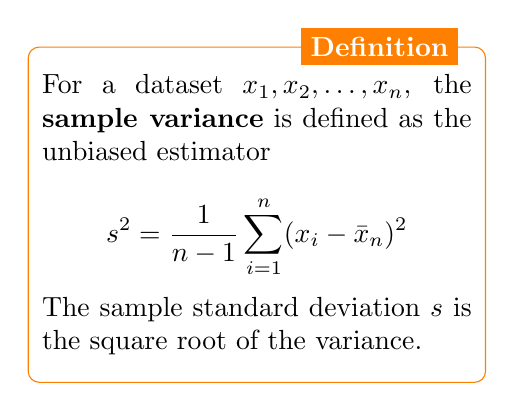
\begin{tikzpicture}
\node [rounded-box] (box){\begin{minipage}{0.45\textwidth}
    For a dataset $x_1, x_2, \dots, x_n$, the \textbf{sample variance} is defined as the unbiased estimator

    $$s^2 = \frac{1}{n-1} \sum_{i=1}^n (x_i - \bar{x}_n)^2$$

    The sample standard deviation $s$ is the square root of the variance.
\end{minipage}};
\node[rounded-box-title, left=10pt] at (box.north east) {Definition};
\end{tikzpicture}

A boxplot and a histogram can be used to visualise a univariate dataset with its statistics and distribution.

A normalised \textbf{histogram} has area equal to one. The height of the bar of a given bin is equal to the proportion of data-points divided by the size of the bin.

\switchcolumn

\subsection{Bivariate Descriptive Statistics}

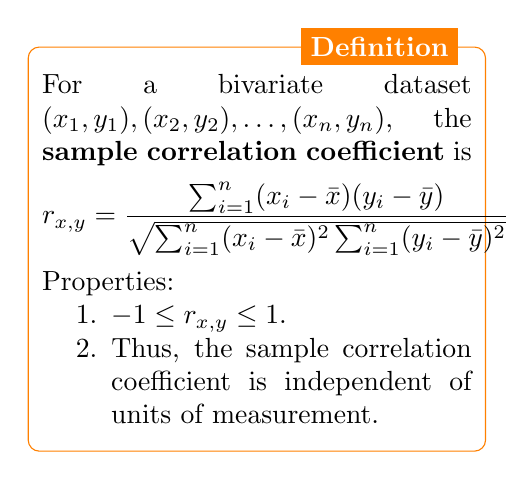
\begin{tikzpicture}
\node [rounded-box] (box){\begin{minipage}{0.45\textwidth}
    For a bivariate dataset $(x_1, y_1), (x_2, y_2), \dots, (x_n, y_n)$, the \textbf{sample correlation coefficient} is

    \vspace{-15pt}

    $$ r_{x, y} = \frac{
    \sum_{i=1}^n (x_i - \bar{x}) (y_i - \bar{y})
    }{\sqrt{
    \sum_{i=1}^n (x_i - \bar{x})^2 \sum_{i=1}^n (y_i - \bar{y})^2
    }} = \frac{s_{xy}}{\sqrt{s_{xx} s_{yy}}}$$

    \vspace{-5pt}

    Properties:

    \begin{enumerate}
        \item $-1 \leq  r_{x, y} \leq 1$.
        \item Thus, the sample correlation coefficient is independent of units of measurement.
    \end{enumerate}
\end{minipage}};
\node[rounded-box-title, left=10pt] at (box.north east) {Definition};
\end{tikzpicture}

A \textbf{scatterplot} can be used to investigate the relationship between two variables.

A \textbf{spurious correlation} is one where there is correlation without causation. A \textbf{latent variable} is an unobserved third variable causing a change in two strongly correlated variables.

\end{paracol}

\begin{verbatim}
data(mtcars)
# View(mtcars)
min(mtcars$wt)
max(mtcars$mpg)
mtcars[mtcars$X == "Duster 360",]
median(c(4, 18, 11, 9, 12, 4, 6, 7))
help(mtcars)
boxplot(mtcars$wt)
round(quantile(mtcars$wt), 3)
round(IQR(mtcars$wt), 3)

data(airquality)
hist(airquality$Temp, breaks=25)
qqnorm(airquality$Temp)
qqline(airquality$Temp, col='red')
hist(airquality$Ozone)
qqnorm(airquality$Ozone)
qqline(airquality$Ozone, col='red')
qqplot(qexp(ppoints(airquality$Ozone)), airquality$Ozone)
qqline(airquality$Ozone, distribution=qexp, col='blue') # not exponential either

set.seed(0)
x <- rnorm(5, mean=0, sd=1)
x
qqnorm(x)
qqline(x, col='red')
# The points are generated randomly from a normal distribution.
# So, it is extremely unlikely that they lie on a straight line.
# When there are more points, small individual deviations do not matter as much,
# and we will be able to draw an almost straight line through the points.

x <- c(3, 5, 7)
y <- c(8, 4, 6)
plot(x, y, xlim = c(0, 10), ylim = c(0, 10), pch = 16, col = "blue", xlab = "x", ylab = "y")
text(x, y, labels = paste("(", x, ",", y, ")", sep = ""), pos = 3)
correlation_coefficient <- cor(x, y)
correlation_coefficient # -0.5

# install.packages("ggplot2movies")
library(ggplot2movies)
data(movies)
plot(movies$year, movies$votes, xlab = "Year", ylab = "Votes")
round(cor(movies$year, movies$votes), 3)

set.seed(0)
x <- rexp(10, 3)
lambda_hat <- 1 / mean(x) # mean = 1 / lambda
round(lambda_hat, 2)
lambda_hat <- log(2) / median(x) # median = log(2) / lambda
round(lambda_hat, 2)
lambda_hat <- sqrt(1 / var(x)) # var = 1 / lambda^2
round(lambda_hat, 2)
set.seed(0)
x <- rexp(100, 3)
lambda_hat <- 1 / mean(x) # mean = 1 / lambda
round(lambda_hat, 2)
lambda_hat <- log(2) / median(x) # median = log(2) / lambda
round(lambda_hat, 2)
lambda_hat <- sqrt(1 / var(x)) # var = 1 / lambda^2
round(lambda_hat, 2)
# The estimates get better as the number of data points increases.

\end{verbatim}
 \newpage
\section{Estimator Theory}

Often, an unknown quantity of interest is represented by some parameter of the model distribution, and one wants to estimate this parameter by means of the observations.

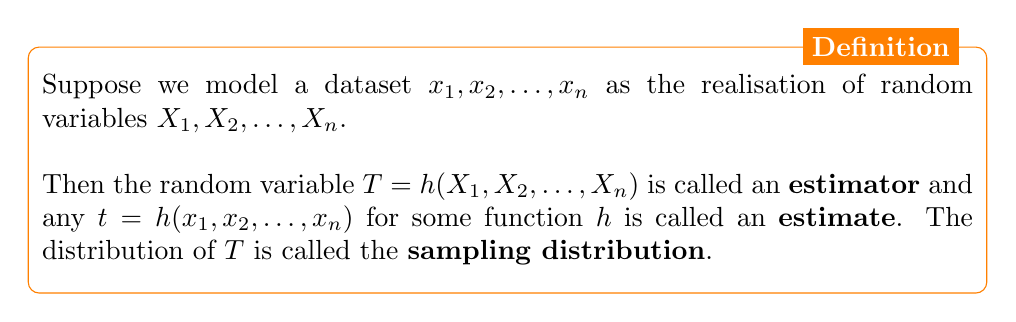
\begin{tikzpicture}
\node [rounded-box] (box){\begin{minipage}{0.975\textwidth}
    Suppose we model a dataset $x_1, x_2, \dots, x_n$ as the realisation of random variables $X_1, X_2, \dots, X_n$. \\

    Then the random variable $T = h(X_1, X_2, \dots, X_n)$ is called an \textbf{estimator} and any $t = h(x_1, x_2, \dots, x_n)$ for some function $h$ is called an \textbf{estimate}. The distribution of $T$ is called the \textbf{sampling distribution}.
\end{minipage}};
\node[rounded-box-title, left=10pt] at (box.north east) {Definition};
\end{tikzpicture}

\begin{paracol}{2}

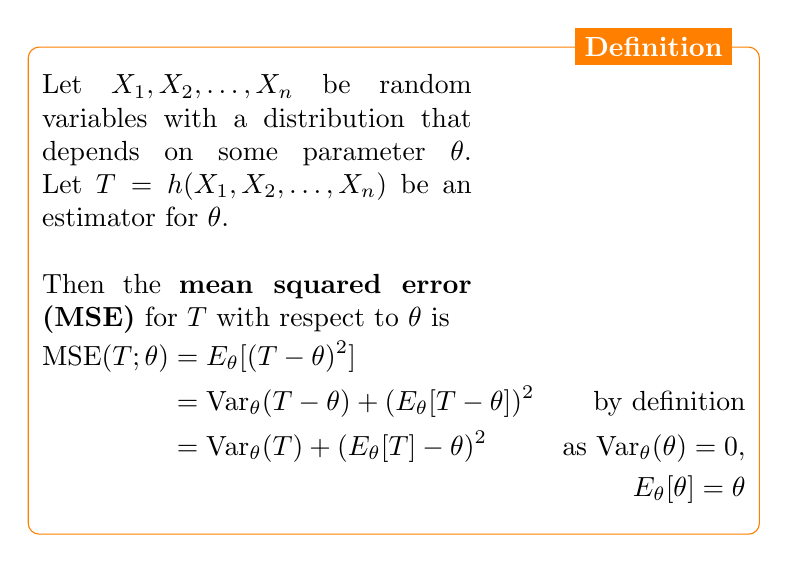
\begin{tikzpicture}
\node [rounded-box] (box){\begin{minipage}{0.45\textwidth}
    Let $X_1, X_2, \dots, X_n$ be random variables with a distribution that depends on some parameter $\theta$. Let $T = h(X_1, X_2, \dots, X_n)$ be an estimator for $\theta$. \\
    
    Then the \textbf{mean squared error (MSE)} for $T$ with respect to $\theta$ is

    \vspace{-20pt}

    \begin{align*}
        \text{MSE}(T; \theta) & = E_\theta[(T - \theta)^2] & \\
        & = \text{Var}_\theta(T - \theta) + (E_\theta[T - \theta])^2 & \text{by definition} \\
        & = \text{Var}_\theta(T) + (E_\theta[T] - \theta)^2 & \text{as Var}_\theta(\theta) = 0, \\
        & & E_\theta[\theta] = \theta
    \end{align*}
\end{minipage}};
\node[rounded-box-title, left=10pt] at (box.north east) {Definition};
\end{tikzpicture}

That is, the MSE is composed of variance and bias:

\begin{itemize}
    \item $\text{Var}_\theta(T)$ measures the variation of $T$ around $E_\theta[T]$,
    \item $E_\theta[T] - \theta$ measures the average deviation of $T$ from $\theta$.
\end{itemize}

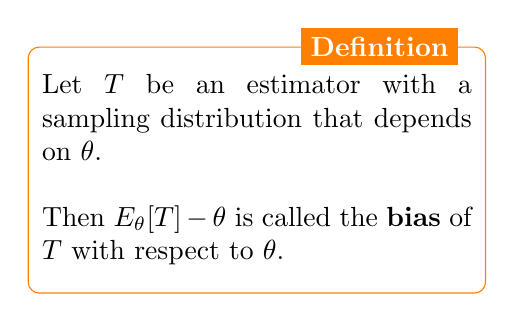
\begin{tikzpicture}
\node [rounded-box] (box){\begin{minipage}{0.45\textwidth}
    Let $T$ be an estimator with a sampling distribution that depends on $\theta$. \\

    Then $E_\theta[T] - \theta$ is called the \textbf{bias} of $T$ with respect to $\theta$.
\end{minipage}};
\node[rounded-box-title, left=10pt] at (box.north east) {Definition};
\end{tikzpicture}

\begin{itemize}
    \item When the bias is positive, the estimator $T$ systematically produces values that are larger than $\theta$.
    \item When the bias is negative, the estimator systematically produces values that are smaller than $\theta$.
    \item Only when the bias is zero, the realisations of $T$ are on average equal to $\theta$.
\end{itemize}

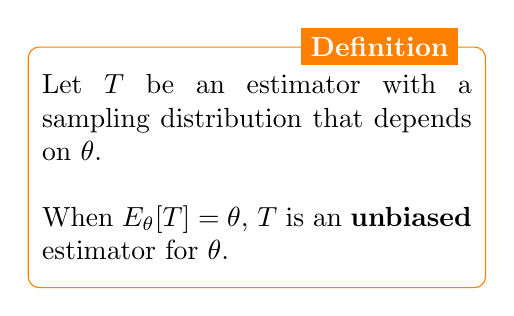
\begin{tikzpicture}
\node [rounded-box] (box){\begin{minipage}{0.45\textwidth}
    Let $T$ be an estimator with a sampling distribution that depends on $\theta$. \\

    When $E_\theta[T] = \theta$, $T$ is an \textbf{unbiased} estimator for $\theta$.
\end{minipage}};
\node[rounded-box-title, left=10pt] at (box.north east) {Definition};
\end{tikzpicture}

\switchcolumn

\textbf{Example}: The sample mean is an unbiased estimator for the mean:

$$E[\bar{X}_n] = E \big[ \frac{1}{n} \sum_{i=1}^n X_i \big] = \frac{1}{n} \sum_{i=1}^n E[X_i] = \frac{1}{n} n \mu = \mu$$

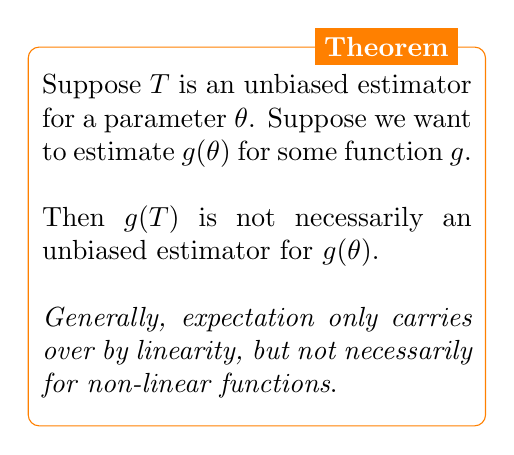
\begin{tikzpicture}
\node [rounded-box] (box){\begin{minipage}{0.45\textwidth}
    Suppose $T$ is an unbiased estimator for a parameter $\theta$. Suppose we want to estimate $g(\theta)$ for some function $g$. \\

    Then $g(T)$ is not necessarily an unbiased estimator for $g(\theta)$. \\
    
    \textit{Generally, expectation only carries over by linearity, but not necessarily for non-linear functions}.
\end{minipage}};
\node[rounded-box-title, left=10pt] at (box.north east) {Theorem};
\end{tikzpicture}

\textbf{Example}: If $T$ is unbiased for $\theta$, $E[T] = \theta$. Then $g(T) = 2 + 3T$ is unbiased for $g(\theta)$: $E[2 + 3T] = 2 + 3 E[T] = 2 + 3 \theta$.

\textbf{Example}: The sample variance is an unbiased estimator for the model variance, but the sample standard deviation is a biased estimator for the model standard deviation:

\begin{align*}
    E[S_n^2] & = \frac{1}{n-1} E \big[ \sum_{i=1}^n (X_i - \bar{X}_n)^2 \big] \\
    & = \frac{1}{n-1} (n-1) \sigma^2 \\
    & = \sigma^2
\end{align*}

By Jensen's inequality, for the convex function $E[S_n^2]$:

$$\sigma^2 = E[S_n^2] > (E[S_n])^2 \Rightarrow E[S_n] < \sigma$$

Thus, $S_n$ has negative bias with respect to $\sigma$.

\end{paracol}

A good estimator should ideally have both low variance and low bias.

Zero bias $E_\theta[T] = \theta$ is a desirable property but \textbf{overall the MSE, composed of variance and bias, determines the performance of an estimator} $T$.

For this reason, in some situations a biased estimator with small variance may be preferable over an unbiased estimator.

Different methods of estimation arise from different principles:

\begin{itemize}
    \item Method of moments: based on the \textit{moments} of the distribution.
    \item Maximum likelihood method: based on the \textit{form} of the distribution.
\end{itemize}

However, although different distributions may have the same moments, the forms of their distributions may be different. For example, the two distinct distributions $X \sim \text{Exp}(1)$ and $Y \sim \mathcal{N}(1, 1)$ both have first and second-order moments $E[X] = 1 = E[Y], \, E[X^2] = 2 = E[Y^2]$.

In such a case, an estimation method based on the form of the distribution (rather than its moments) provides more information; and likely a better estimator (with a lower MSE).

\subsection{The Method of Moments}

\begin{paracol}{2}

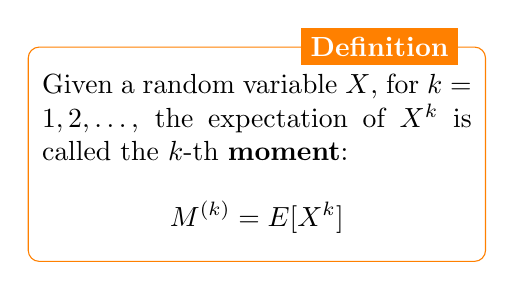
\begin{tikzpicture}
\node [rounded-box] (box){\begin{minipage}{0.45\textwidth}
    Given a random variable $X$, for $k = 1, 2, \dots$, the expectation of $X^k$ is called the $k$-th \textbf{moment}:

    $$M^{(k)} = E[X^k]$$
\end{minipage}};
\node[rounded-box-title, left=10pt] at (box.north east) {Definition};
\end{tikzpicture}

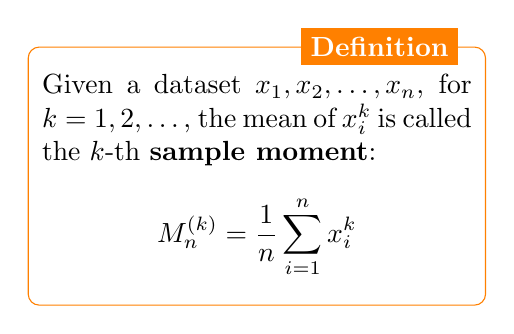
\begin{tikzpicture}
\node [rounded-box] (box){\begin{minipage}{0.45\textwidth}
    Given a dataset $x_1, x_2, \dots, x_n$, for $k = 1, 2, \dots$, the mean of $x_i^k$ is called the $k$-th \textbf{sample moment}:

    $$M_n^{(k)} = \frac{1}{n} \sum_{i=1}^n x_i^k$$
\end{minipage}};
\node[rounded-box-title, left=10pt] at (box.north east) {Definition};
\end{tikzpicture}

\textbf{Example}: If $X \sim \mathcal{N}(\mu, \sigma^2)$, then

\vspace{-20pt}

\begin{align*}
    \sigma^2 = \text{Var}(X) & = E[X^2] - (E[X])^2 \\
    & = \frac{1}{n} \sum_{i=1}^n x_i^2 - \Bigg( \frac{1}{n} \sum_{i=1}^n x_i \Bigg)^2 \\
    & = \frac{1}{n} \sum_{i=1}^n (x_i - \bar{x}_n)^2
\end{align*}

(Note: The \textit{sample} variance is commonly divided by $(n-1)$ so it will be an unbiased estimator.)

\switchcolumn

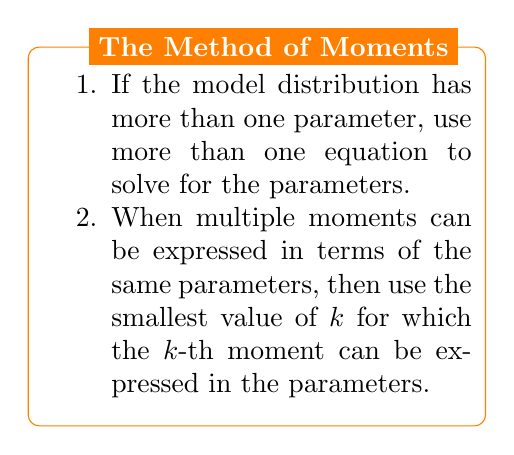
\begin{tikzpicture}
\node [rounded-box] (box){\begin{minipage}{0.45\textwidth}
    \begin{enumerate}
        \item If the model distribution has more than one parameter, use more than one equation to solve for the parameters.
        \item When multiple moments can be expressed in terms of the same parameters, then use the smallest value of $k$ for which the $k$-th moment can be expressed in the parameters.
    \end{enumerate}
\end{minipage}};
\node[rounded-box-title, left=10pt] at (box.north east) {The Method of Moments};
\end{tikzpicture}

\textbf{Example}: $X_1, X_2, \dots, X_n \sim \mathcal{N}(\mu, \sigma^2)$ has two parameters:

$$\frac{1}{n} \sum_{i=1}^n x_i = E[X_1] = \mu \quad \Rightarrow \quad \hat{\mu} = \bar{X}_n$$

\vspace{-20pt}

\begin{align*}
    \frac{1}{n} \sum_{i=1}^n x_i^2 & = E[X_1^2] = \text{Var}(X_1) + (E[X_1])^2 = \sigma^2 + \mu^2 \\
    \Rightarrow \quad \hat{\sigma}^2 & = \frac{1}{n} \sum_{i=1}^n X_i^2 - \hat{\mu} = \frac{1}{n} \sum_{i=1}^n X_i^2 - \bar{X}_n = \frac{1}{n} \sum_{i=1}^n (X_i - \bar{X}_n)^2
\end{align*}

\textbf{Example}: $X_1, X_2, \dots, X_n \sim \mathcal{N}(0, \sigma^2)$ has one parameter, but the first moment is zero: $E[X_1] = 0$.

\vspace{-20pt}

$$E[X_1^2] = \text{Var}(X_1) + (E[X_1])^2 = \sigma^2 + 0
\quad \Rightarrow \quad
\hat{\sigma} = \sqrt{\frac{1}{n} \sum_{i=1}^n X_i^2}$$

\end{paracol}

\vspace{-10pt}

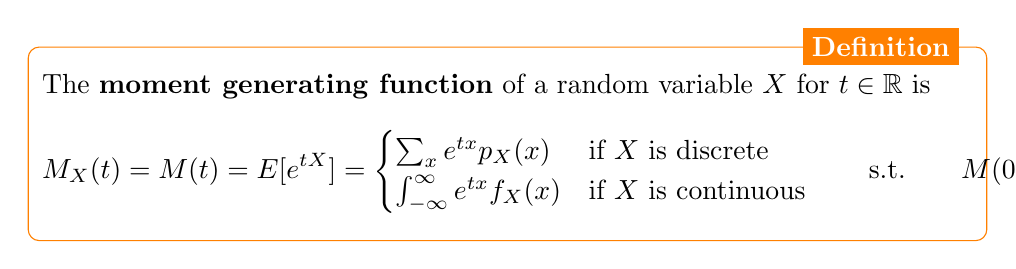
\begin{tikzpicture}
\node [rounded-box] (box){\begin{minipage}{0.975\textwidth}
    The \textbf{moment generating function} of a random variable $X$ for $t \in \mathbb{R}$ is

    \vspace{-10pt}

    $$M_X(t) = M(t) = E[e^{tX}] = \begin{cases}
        \sum_x e^{tx} p_X(x) & \text{if } X \text{ is discrete} \\

        \int_{-\infty}^\infty e^{tx} f_X(x) & \text{if } X \text{ is continuous}
    \end{cases} \qquad \text{s.t.} \qquad M(0) = 1  = \begin{cases}
        \sum_x p_X(x) & \text{if } X \text{ is discrete} \\

        \int_{-\infty}^\infty f_X(x) & \text{if } X \text{ is continuous}
    \end{cases}$$
\end{minipage}};
\node[rounded-box-title, left=10pt] at (box.north east) {Definition};
\end{tikzpicture}

\begin{paracol}{2}

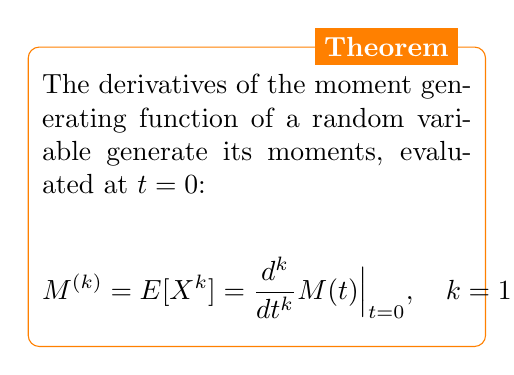
\begin{tikzpicture}
\node [rounded-box] (box){\begin{minipage}{0.45\textwidth}
    The derivatives of the moment generating function of a random variable generate its moments, evaluated at $t = 0$:

    $$M^{(k)} = E[X^k] = \frac{d^k}{dt^k} M(t) \Big|_{t=0}, \quad k = 1, 2, 3, \dots$$
\end{minipage}};
\node[rounded-box-title, left=10pt] at (box.north east) {Theorem};
\end{tikzpicture}

\switchcolumn

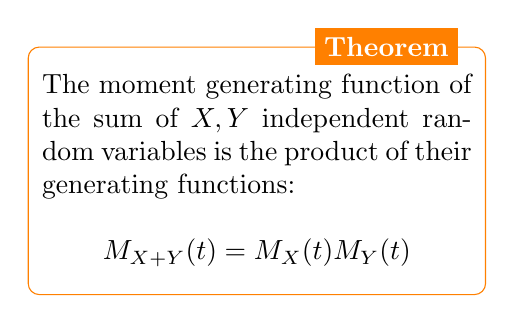
\begin{tikzpicture}
\node [rounded-box] (box){\begin{minipage}{0.45\textwidth}
    The moment generating function of the sum of $X, Y$ independent random variables is the product of their generating functions:

    $$M_{X + Y}(t) = M_X(t) M_Y(t)$$
\end{minipage}};
\node[rounded-box-title, left=10pt] at (box.north east) {Theorem};
\end{tikzpicture}

\end{paracol}

\textbf{Examples}: $E[X] = M'(0), \quad \text{Var}(X) = M''(0) - M'(0)^2$

$\text{Ber}(p): M(t) = p e^t + 1 - p, \quad \text{Bin}(n, p): M(t) = (p e^t + 1 - p)^2, \quad \mathcal{N}(\mu, \sigma^2): M(t) = e^{t \mu + t^2 \sigma^2 / 2}$

\subsection{The Maximum Likelihood Method}

\begin{paracol}{2}

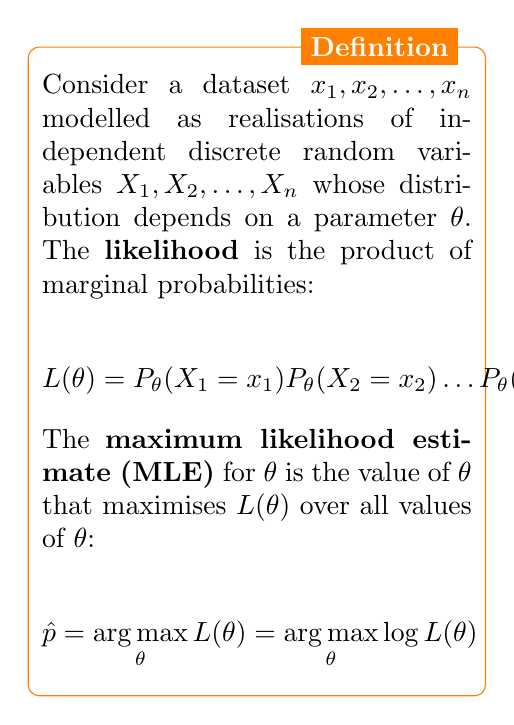
\begin{tikzpicture}
\node [rounded-box] (box){\begin{minipage}{0.45\textwidth}
    Consider a dataset $x_1, x_2, \dots, x_n$ modelled as realisations of independent discrete random variables $X_1, X_2, \dots, X_n$ whose distribution depends on a parameter $\theta$. The \textbf{likelihood} is the product of marginal probabilities:

    $$L(\theta) = P_\theta(X_1 = x_1) P_\theta(X_2 = x_2) \dots P_\theta(X_n = x_n)$$

    The \textbf{maximum likelihood estimate (MLE)} for $\theta$ is the value of $\theta$ that maximises $L(\theta)$ over all values of $\theta$:

    $$\hat{p} = \operatorname*{arg\,max}_\theta{L(\theta)} = \operatorname*{arg\,max}_\theta{\log L(\theta)}$$
\end{minipage}};
\node[rounded-box-title, left=10pt] at (box.north east) {Definition};
\end{tikzpicture}

(In practice, maximising $\log L(\theta)$ is often easier.)

\switchcolumn

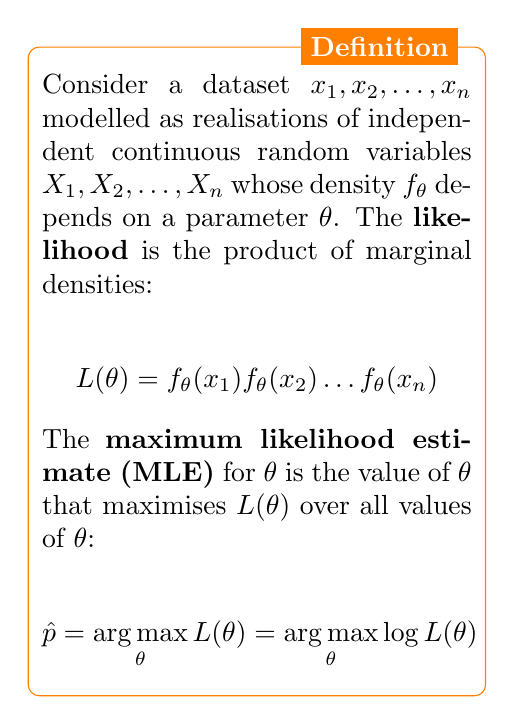
\begin{tikzpicture}
\node [rounded-box] (box){\begin{minipage}{0.45\textwidth}
    Consider a dataset $x_1, x_2, \dots, x_n$ modelled as realisations of independent continuous random variables $X_1, X_2, \dots, X_n$ whose density $f_\theta$ depends on a parameter $\theta$. The \textbf{likelihood} is the product of marginal densities:

    $$L(\theta) = f_\theta(x_1) f_\theta(x_2) \dots f_\theta(x_n)$$

    The \textbf{maximum likelihood estimate (MLE)} for $\theta$ is the value of $\theta$ that maximises $L(\theta)$ over all values of $\theta$:

    $$\hat{p} = \operatorname*{arg\,max}_\theta{L(\theta)} = \operatorname*{arg\,max}_\theta{\log L(\theta)}$$
\end{minipage}};
\node[rounded-box-title, left=10pt] at (box.north east) {Definition};
\end{tikzpicture}

In general it is often true that the maximum likelihood estimator has the lowest MSE (for large $n$), of the asymptotically unbiased estimators.

\end{paracol}

\newpage

\begin{verbatim}set.seed(0)
n <- 10
n_exp <- 10000
# Estimator based on variance
K_hat_var <- 1:n_exp
for (i in 1:n_exp) {
  x <- sample(1:1000, n, replace=FALSE)
  K_hat_var[i] <- sqrt(12 * var(x) + 1)
}
mean(K_hat_var)
var(K_hat_var)
# Estimator based on median
K_hat_median <- 1:n_exp
for (i in 1:n_exp) {
  x <- sample(1:1000, n)
  K_hat_median[i] <- 2 * median(x) - 1
}
mean(K_hat_median)
var(K_hat_median)
# Estimator based on mean
K_hat_mean <- 1:n_exp
for (i in 1:n_exp) {
  x <- sample(1:1000, n)
  K_hat_mean[i] <- 2 * mean(x) - 1
}
mean(K_hat_mean)
var(K_hat_mean)
# Plot estimators
hist(K_hat_var, col='green', breaks=seq(0, 2000, 100), density=50)
hist(K_hat_median, col='red', breaks=seq(0, 2000, 100), density=50, add=TRUE)
hist(K_hat_mean, col='blue', breaks=seq(0, 2000, 100), density=50, add=TRUE)
# Why is the estimator based on the median different from the estimator based on the average, even though
# their theoretical values are the same?
# The estimators happen to have the same expectation, but they are different random variables.

m <- 500
n <- 100
p <- 0.5
N <- 1000
T1 <- 1:N
T2 <- 1:N
for (i in 1:N) {
  X <- rbinom(m, size=1, prob=p)
  Y <- rbinom(n, size=1, prob=p)

  T1[i] <- (mean(X) + mean(Y)) / 2
  T2[i] <- (sum(X) + sum(Y)) / (m + n)
}
mean(T1)
mean(T2)
MSE_T1 <- mean((p - T1)^2)
MSE_T2 <- mean((p - T2)^2)
MSE_T1
MSE_T2
# Smaller MSE gives a better estimator.

\end{verbatim}
 \newpage
\section{Hypothesis Testing}

\begin{paracol}{2}

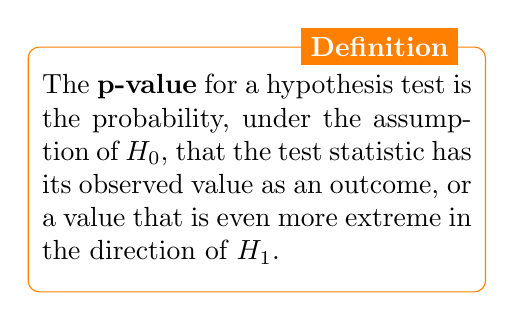
\begin{tikzpicture}
\node [rounded-box] (box){\begin{minipage}{0.45\textwidth}
    The \textbf{p-value} for a hypothesis test is the probability, under the assumption of $H_0$, that the test statistic has its observed value as an outcome, or a value that is even more extreme in the direction of $H_1$.
\end{minipage}};
\node[rounded-box-title, left=10pt] at (box.north east) {Definition};
\end{tikzpicture}

A small p-value  implies that random variation because of the sampling process alone is not likely to account for the observed difference.

Therefore, with a small p-value, we reject $H_0$:

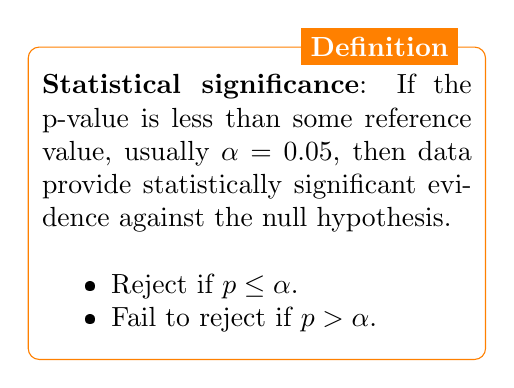
\begin{tikzpicture}
\node [rounded-box] (box){\begin{minipage}{0.45\textwidth}
    \textbf{Statistical significance}: If the p-value is less than some reference value, usually $\alpha = 0.05$, then data provide statistically significant evidence against the null hypothesis. \\

    \begin{itemize}
        \item Reject if $p \leq \alpha$.
        \item Fail to reject if $p > \alpha$.
    \end{itemize}
\end{minipage}};
\node[rounded-box-title, left=10pt] at (box.north east) {Definition};
\end{tikzpicture}

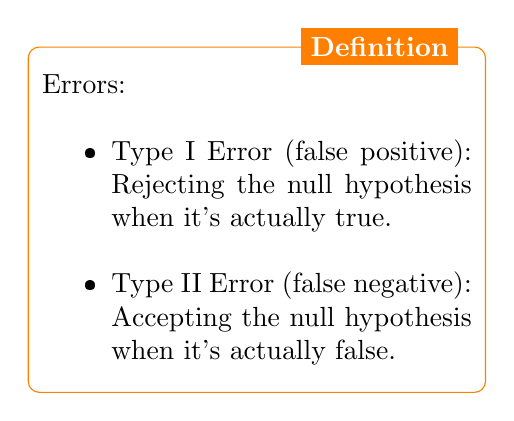
\begin{tikzpicture}
\node [rounded-box] (box){\begin{minipage}{0.45\textwidth}
    Errors: \\

    \begin{itemize}
        \item Type I Error (false positive): Rejecting the null hypothesis when it's actually true. \\

        \item Type II Error (false negative): Accepting the null hypothesis when it's actually false.
    \end{itemize}
\end{minipage}};
\node[rounded-box-title, left=10pt] at (box.north east) {Definition};
\end{tikzpicture}

\switchcolumn

By reducing the rate of one type of error, you risk increasing the rate of the other type.

But with more and better data it is possible to reduce both error rates simultaneously.

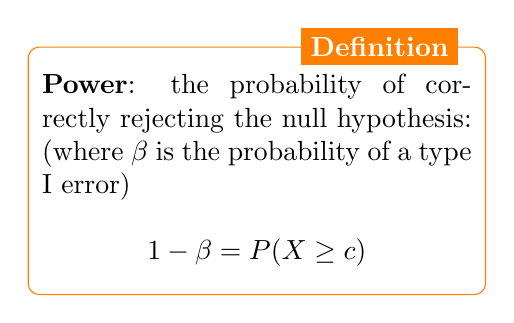
\begin{tikzpicture}
\node [rounded-box] (box){\begin{minipage}{0.45\textwidth}
    \textbf{Power}: the probability of correctly rejecting the null hypothesis: (where $\beta$ is the probability of a type I error)

    $$1 - \beta = P(X \geq c)$$
\end{minipage}};
\node[rounded-box-title, left=10pt] at (box.north east) {Definition};
\end{tikzpicture}

\textbf{Example}: Suppose you are given a number $v$, which is a realisation of a random variable $V \sim \mathcal{N}(\mu, 1)$. Consider the following hypotheses: $H_0: \mu = 0, H_1: \mu\neq 0$. You decide to reject $H_0$ when $|v| \geq 2.5$.

The probability of committing a type I error is $P(|V| \geq 2.5) = P(V \leq -2.5) + P(V \geq 2.5) = 2 \cdot P(V \leq -2.5) = 2 \cdot P \big( \frac{V - \mu}{\sigma} \leq \frac{-2.5 - \mu}{\sigma} \big) = 2 = P \big( Z \leq \frac{-2.5-0}{1} \big) = 2 \cdot P(Z \leq -2.5) = 2 \cdot 0.0062 = 0.0124$. \\

A z-score measures the number of standard deviations that a datapoint $x$ is from the mean $\mu$.

\begin{itemize}
    \item When $x$ is 1 standard deviation larger than the mean, then $z = 1$.
    \item When $x$ is 2 standard deviations smaller than the mean, then $z = -2$.
\end{itemize}

\end{paracol}

\subsection{The One-Sample t-Test}

\begin{paracol}{2}

Let $H_0: \mu = \mu_0, H_1: \mu \neq \mu_0$ for some $\mu_0$. Since $\bar{X}_n \approx \mu$ by the LLN, so $|| \bar{X}_n - \mu_0 || \approx 0$ is in favour of the null hypothesis and $|| \bar{X}_n - \mu_0 || \gg 0$ is in favour of the alternative hypothesis.

However, a difference is not a representative test statistic unless it is compared with something - the standard deviation:

\begin{align*}
    \sqrt{\text{Var}(\bar{X}_n - \mu_0)} & = \sqrt{\text{Var}(\bar{X}_n)} = \sqrt{\text{Var}\Big( \frac{1}{n} \sum_{i=1}^n X_i \Big)} & \\
    & = \sqrt{\frac{1}{n^2} \sum_{i=1}^n \text{Var}(X_i)} \qquad \text{for independent $X_i$} \\
    & = \sqrt{\frac{1}{n^2} n \sigma^2} & \\
    & = \frac{\sigma}{\sqrt{n}}
\end{align*}

Because the true value of $\sigma$ is unknown, it is replaced by the sample standard deviation $\frac{S_n}{\sqrt{n}}$, where $S_n^2 = \frac{1}{n-1} \sum_{i=1}^n (X_i - \bar{X}_n)^2$.

\switchcolumn

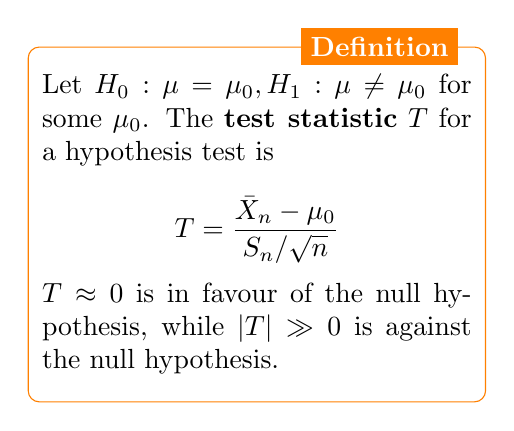
\begin{tikzpicture}
\node [rounded-box] (box){\begin{minipage}{0.45\textwidth}
    Let $H_0: \mu = \mu_0, H_1: \mu \neq \mu_0$ for some $\mu_0$. The \textbf{test statistic} $T$ for a hypothesis test is

    $$T = \frac{\bar{X}_n - \mu_0}{S_n / \sqrt{n}}$$

    $T \approx 0$ is in favour of the null hypothesis, while $| T | \gg 0$ is against the null hypothesis.
\end{minipage}};
\node[rounded-box-title, left=10pt] at (box.north east) {Definition};
\end{tikzpicture}

Since independent $X_1, X_2, \dots, X_n \sim \mathcal{N}(\mu, \sigma^2)$, the sample mean $\bar{X}_n \sim \mathcal{N}\big( \mu, \frac{\sigma^2}{n} \big)$ and the hypothetical test statistic $\frac{\bar{X}_n - \mu_0}{\sigma \ \sqrt{n}} \sim \mathcal{N}(0, 1)$.

\switchcolumn

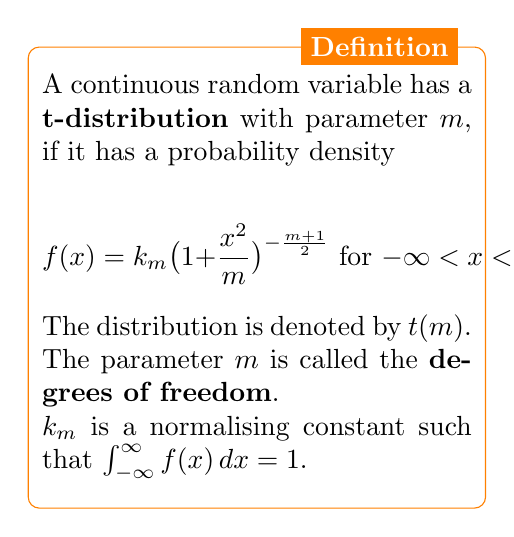
\begin{tikzpicture}
\node [rounded-box] (box){\begin{minipage}{0.45\textwidth}
    A continuous random variable has a $\mathbf{t}$\textbf{-distribution} with parameter $m$, if it has a probability density

    $$f(x) = k_m \big( 1 + \frac{x^2}{m} \big)^{-\frac{m+1}{2}} \text{ for } -\infty < x < \infty$$

    The distribution is denoted by $t(m)$. The parameter $m$ is called the \textbf{degrees of freedom}.

    $k_m$ is a normalising constant such that $\int_{-\infty}^\infty f(x) \,dx = 1$.
\end{minipage}};
\node[rounded-box-title, left=10pt] at (box.north east) {Definition};
\end{tikzpicture}

\begin{itemize}
    \item When $m = 1$, the distribution equals the Cauchy distribution:

    $$f(x) = \frac{1}{\pi} (1 + x^2)^{-1}$$

    \item As $m \rightarrow \infty$, the distribution approaches a Normal distribution:

    $$f(x) \rightarrow \frac{1}{\sqrt{2 \pi}} e^{-x^2/2}$$
\end{itemize}

Therefore, a t-distribution is somewhere between these two extremes. The density is symmetric around zero and it is bell-shaped like the standard normal. The distinguishing feature is that densities of the t-distribution have heavier tails - the mean is smaller and the density goes to zero more slowly than the standard normal density as $s \rightarrow \pm \infty$.

\switchcolumn

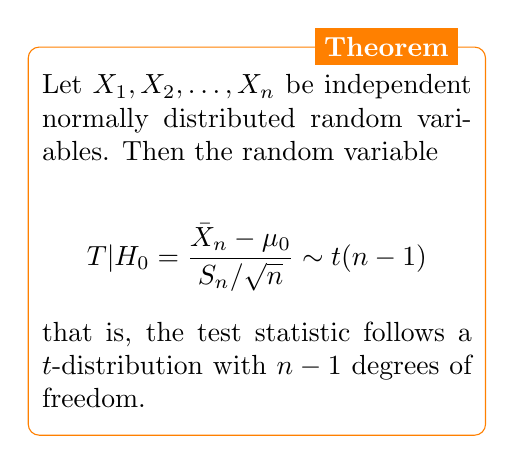
\begin{tikzpicture}
\node [rounded-box] (box){\begin{minipage}{0.45\textwidth}
    Let $X_1, X_2, \dots, X_n$ be independent normally distributed random variables. Then the random variable

    $$T | H_0 = \frac{\bar{X}_n - \mu_0}{S_n / \sqrt{n}} \sim t(n-1)$$

    that is, the test statistic follows a $t$-distribution with $n-1$ degrees of freedom.
\end{minipage}};
\node[rounded-box-title, left=10pt] at (box.north east) {Theorem};
\end{tikzpicture}

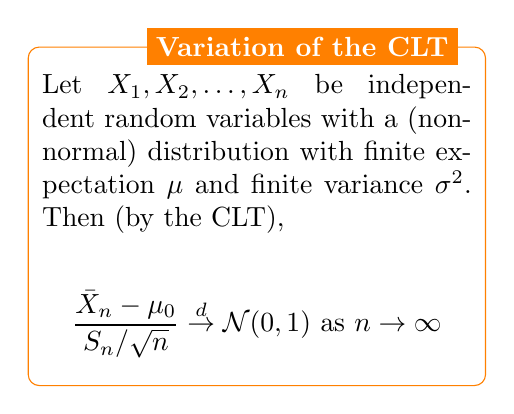
\begin{tikzpicture}
\node [rounded-box] (box){\begin{minipage}{0.45\textwidth}
    Let $X_1, X_2, \dots, X_n$ be independent random variables with a (non-normal) distribution with finite expectation $\mu$ and finite variance $\sigma^2$. Then (by the CLT),

    $$\frac{\bar{X}_n - \mu_0}{S_n / \sqrt{n}} \overset{d}{\rightarrow} \mathcal{N}(0, 1) \text{ as } n \rightarrow \infty$$
\end{minipage}};
\node[rounded-box-title, left=10pt] at (box.north east) {Variation of the CLT};
\end{tikzpicture}

Consequently,

$$P \Big( a < \frac{\bar{X}_n - \mu_0}{S_n / \sqrt{n}} < b \Big) \rightarrow P(a < Z < b),
\quad
Z \sim \mathcal{N}(0, 1)$$

\end{paracol}

\subsection{Two-Sample Testing}

\begin{paracol}{2}

One-sample $t$-test: $T = \frac{\bar{X}_n}{(S_n / \sqrt{n}} \sim t(n-1)$

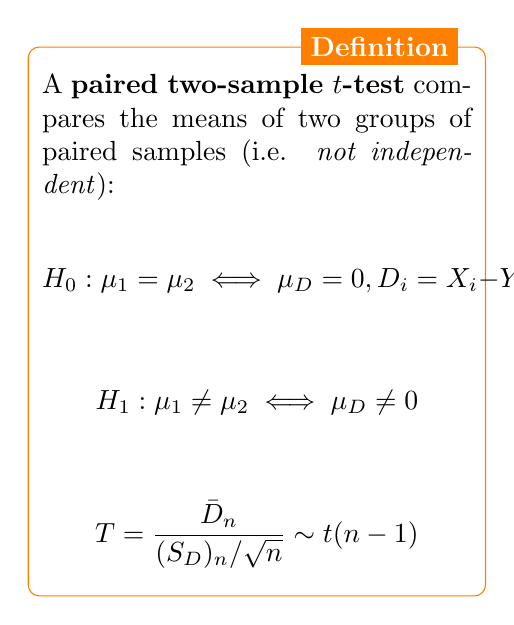
\begin{tikzpicture}
\node [rounded-box] (box){\begin{minipage}{0.45\textwidth}
    A \textbf{paired two-sample $t$-test} compares the means of two groups of paired samples (i.e. \textit{not independent}):
    
    $$H_0: \mu_1 = \mu_2 \iff \mu_D = 0, D_i = X_i - Y_i$$
    
    $$H_1: \mu_1 \neq \mu_2 \iff \mu_D \neq 0$$
    
    $$T = \frac{\bar{D}_n}{(S_D)_n / \sqrt{n}} \sim t(n-1)$$
\end{minipage}};
\node[rounded-box-title, left=10pt] at (box.north east) {Definition};
\end{tikzpicture}

\textbf{Examples}:

\begin{itemize}
    \item Blood pressure of patients before and after a treatment
    \item Market capitalisation of companies now and in two years
    \item Air resistance of an airplane wing before and after a coating is applied
    \item Lung closing capacity for smokers and non-smokers
\end{itemize}

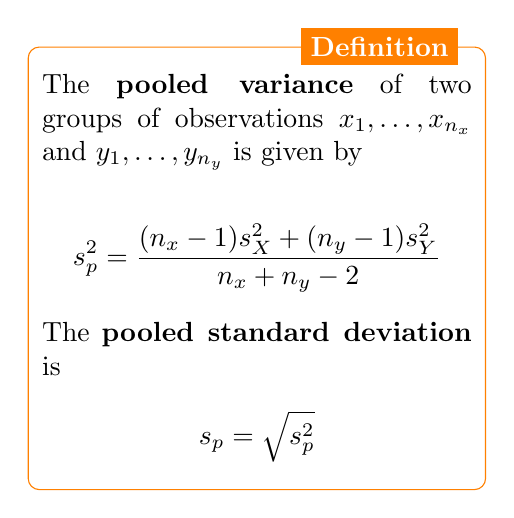
\begin{tikzpicture}
\node [rounded-box] (box){\begin{minipage}{0.45\textwidth}
    The \textbf{pooled variance} of two groups of observations $x_1, \dots, x_{n_x}$ and $y_1, \dots, y_{n_y}$ is given by

    $$s_p^2 = \frac{(n_x - 1) s_X^2 + (n_y - 1) s_Y^2}{n_x + n_y - 2}$$

    The \textbf{pooled standard deviation} is

    $$s_p = \sqrt{s_p^2}$$
\end{minipage}};
\node[rounded-box-title, left=10pt] at (box.north east) {Definition};
\end{tikzpicture}

\switchcolumn

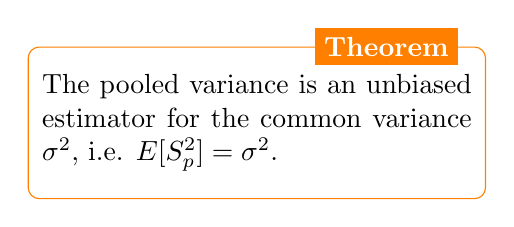
\begin{tikzpicture}
\node [rounded-box] (box){\begin{minipage}{0.45\textwidth}
    The pooled variance is an unbiased estimator for the common variance $\sigma^2$, i.e. $E[S_p^2] = \sigma^2$.
\end{minipage}};
\node[rounded-box-title, left=10pt] at (box.north east) {Theorem};
\end{tikzpicture}

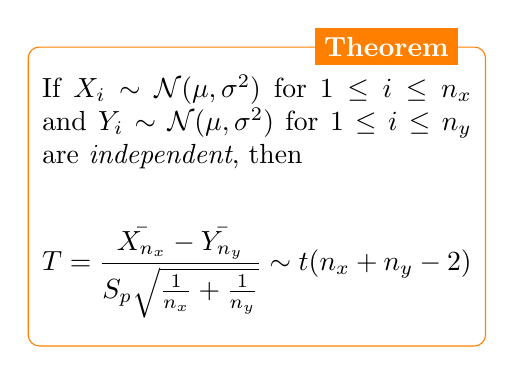
\begin{tikzpicture}
\node [rounded-box] (box){\begin{minipage}{0.45\textwidth}
    If $X_i \sim \mathcal{N}(\mu, \sigma^2)$ for $1 \leq i \leq n_x$ and $Y_i \sim \mathcal{N}(\mu, \sigma^2)$ for $1 \leq i \leq n_y$ are \textit{independent}, then

    $$T = \frac{\bar{X_{n_x}} - \bar{Y_{n_y}}}{S_p \sqrt{\frac{1}{n_x} + \frac{1}{n_y}}} \sim t(n_x + n_y - 2)$$
\end{minipage}};
\node[rounded-box-title, left=10pt] at (box.north east) {Theorem};
\end{tikzpicture}

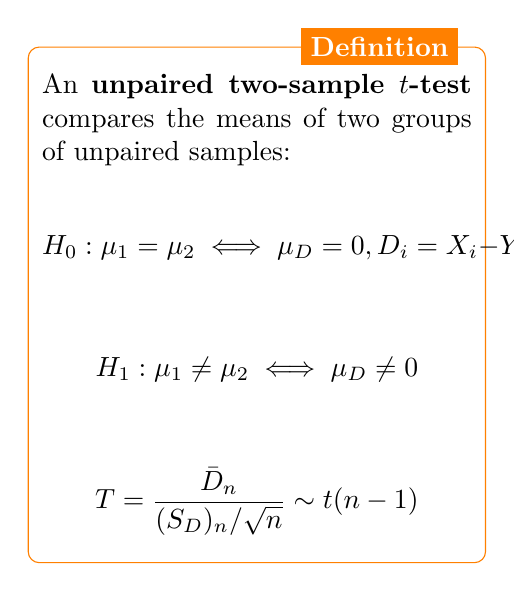
\begin{tikzpicture}
\node [rounded-box] (box){\begin{minipage}{0.45\textwidth}
    An \textbf{unpaired two-sample $t$-test} compares the means of two groups of unpaired samples:
    
    $$H_0: \mu_1 = \mu_2 \iff \mu_D = 0, D_i = X_i - Y_i$$
    
    $$H_1: \mu_1 \neq \mu_2 \iff \mu_D \neq 0$$
    
    $$T = \frac{\bar{D}_n}{(S_D)_n / \sqrt{n}} \sim t(n-1)$$
\end{minipage}};
\node[rounded-box-title, left=10pt] at (box.north east) {Definition};
\end{tikzpicture}

If the two samples have different variances, \textbf{Welch's test} can be applied.

\end{paracol}

\newpage

\begin{verbatim}
set.seed(42)

# Suppose you toss a fair coin 10 times. To compute the probability of a certain
# number of heads, you can use the command dbinom. It returns the value of the
# probability mass function at that number.
dbinom(5, size=10, prob=0.5)

# To compute the probability of computing at most a certain number of heads, you
# can use the command pbinom. It returns the value of the cumulative density
# function at that number. What is the probability of at most 6 and at least 3?
pbinom(6, size=10, prob=0.5) - pbinom(2, size=10, prob=0.5)

dbinom(500, size=1000, prob=0.5)
range <- 425:575
plot(range, dbinom(range, size=1000, prob=0.5))
plot(range, pbinom(range, size=1000, prob=0.5))
# To compute the number of heads, such that the probability of flipping that many
# heads has a certain value, you can use the command qbinom. It returns the value
# of the inverse cumulative density function or quantile function at that probability.
# The first quartile (Q1) is the point where you expect the cumulative density function to be 0.25.
qbinom(0.25, size=1000, prob=0.5)

# To draw random samples of the binomial distribution, you can use the command rbinom.
# Flip 1000 coins 10 times. What is the mean?
rsample <- rbinom(10, size=1000, prob=0.5)
mean(rsample)

# What's the probability of 133 successes in 175 trials?
dbinom(133, size=175, prob=0.68)
range <- 85:150
plot(range, dbinom(range, size=175, prob=0.68))
# What's the probability of at least 133 successes?
1 - pbinom(132, size=175, prob=0.68)
# This is the p-value for hypotheses H_0: mu=0.68, H_1: mu > 0.68
binom.test(133, n=175, p=0.68, alternative = "greater", conf.level = 0.95)

data("iris")
head(iris)
only_versicolor <- iris[iris$Species == "versicolor",]
sep_len <- only_versicolor$Sepal.Length
hist(sep_len)
qqnorm(sep_len)
t.test(sep_len, mu=5.731)

data("chickwts")
sunfl <- subset(chickwts, feed == "sunflower")[,1]
soyb <- subset(chickwts, feed == "soybean")[,1]
var.test(sunfl, soyb)
# The high p-value tells you not to reject the equality of variances.
# This means we now know which t-test to apply: the two-sample unpaired t-test, equal variances.
t.test(sunfl, soyb, alternative = "greater", paired = FALSE, var.equal = TRUE)

\end{verbatim}
 \newpage
\section{Confidence Intervals}

\begin{paracol}{2}

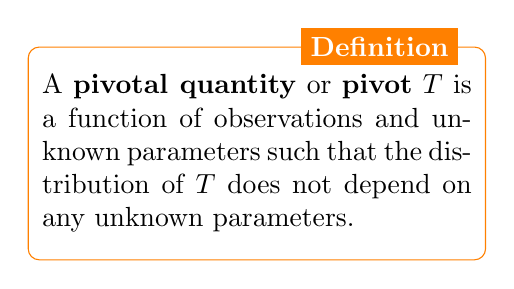
\begin{tikzpicture}
\node [rounded-box] (box){\begin{minipage}{0.45\textwidth}
    A \textbf{pivotal quantity} or \textbf{pivot} $T$ is a function of observations and unknown parameters such that the distribution of $T$ does not depend on any unknown parameters.
\end{minipage}};
\node[rounded-box-title, left=10pt] at (box.north east) {Definition};
\end{tikzpicture}

\textbf{Example}: The test statistic $T = \frac{\bar{X}_n - \mu}{S_n \ \sqrt{n}} \sim t(n-1)$ depends both on observations and unknown parameters, while its distribution does not. $T$ is a pivot.

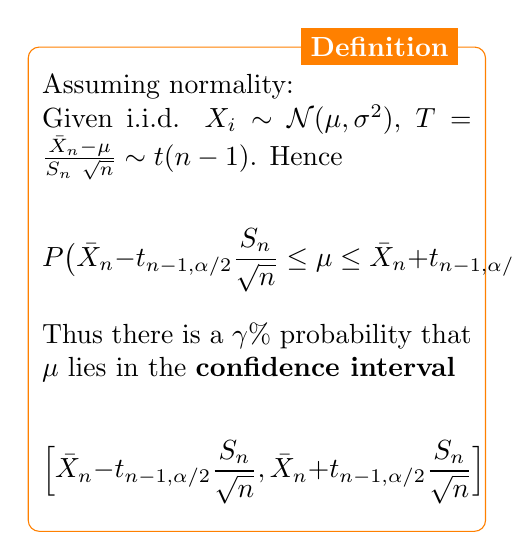
\begin{tikzpicture}
\node [rounded-box] (box){\begin{minipage}{0.45\textwidth}
    Assuming normality:

    Given i.i.d. $X_i \sim \mathcal{N}(\mu, \sigma^2)$, $T = \frac{\bar{X}_n - \mu}{S_n \ \sqrt{n}} \sim t(n-1)$. Hence

    $$P \big(\bar{X}_n - t_{n-1, \alpha / 2} \frac{S_n}{\sqrt{n}} \leq \mu \leq \bar{X}_n + t_{n-1, \alpha / 2} \frac{S_n}{\sqrt{n}} \big) = 1 - \alpha = \gamma$$

    Thus there is a $\gamma \%$ probability that $\mu$ lies in the \textbf{confidence interval}

    $$\Big[ \bar{X}_n - t_{n-1, \alpha / 2} \frac{S_n}{\sqrt{n}} , \bar{X}_n + t_{n-1, \alpha / 2} \frac{S_n}{\sqrt{n}} \Big]$$
\end{minipage}};
\node[rounded-box-title, left=10pt] at (box.north east) {Definition};
\end{tikzpicture}

NB: The statement "$\mu$ has $\gamma \%$ probability of lying in this interval" is not correct!

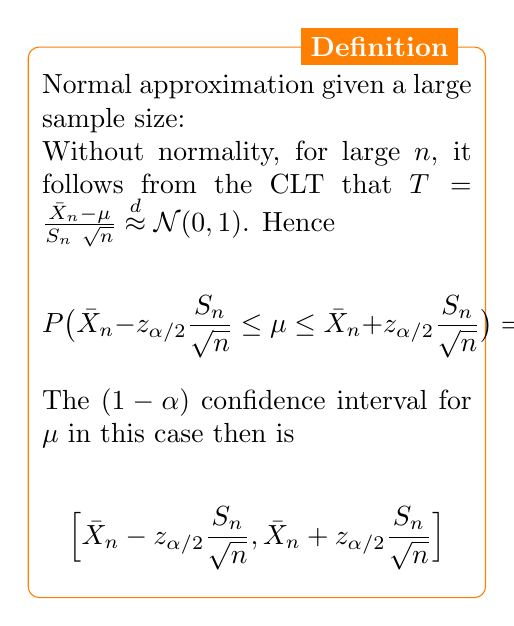
\begin{tikzpicture}
\node [rounded-box] (box){\begin{minipage}{0.45\textwidth}
    Normal approximation given a large sample size:

    Without normality, for large $n$, it follows from the CLT that $T = \frac{\bar{X}_n - \mu}{S_n \ \sqrt{n}} \overset{d}{\approx} \mathcal{N}(0, 1)$. Hence

    $$P \big(\bar{X}_n - z_{\alpha / 2} \frac{S_n}{\sqrt{n}} \leq \mu \leq \bar{X}_n + z_{\alpha / 2} \frac{S_n}{\sqrt{n}} \big) = 1 - \alpha = \gamma$$

    The $(1 - \alpha)$ confidence interval for $\mu$ in this case then is

    $$\Big[ \bar{X}_n - z_{\alpha / 2} \frac{S_n}{\sqrt{n}} , \bar{X}_n + z_{\alpha / 2} \frac{S_n}{\sqrt{n}} \Big]$$
\end{minipage}};
\node[rounded-box-title, left=10pt] at (box.north east) {Definition};
\end{tikzpicture}

\textbf{Disadvantages of the CLT approximation}:

\begin{enumerate}
    \item The CLT only gives an approximate interval.
    \item The approximation may not be very good for small $n$.
    \item It is more accurate to use the \textit{actual distribution}.
\end{enumerate}

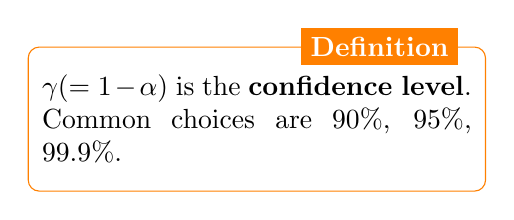
\begin{tikzpicture}
\node [rounded-box] (box){\begin{minipage}{0.45\textwidth}
    $\gamma (= 1 - \alpha)$ is the \textbf{confidence level}. Common choices are 90\%, 95\%, 99.9\%.
\end{minipage}};
\node[rounded-box-title, left=10pt] at (box.north east) {Definition};
\end{tikzpicture}

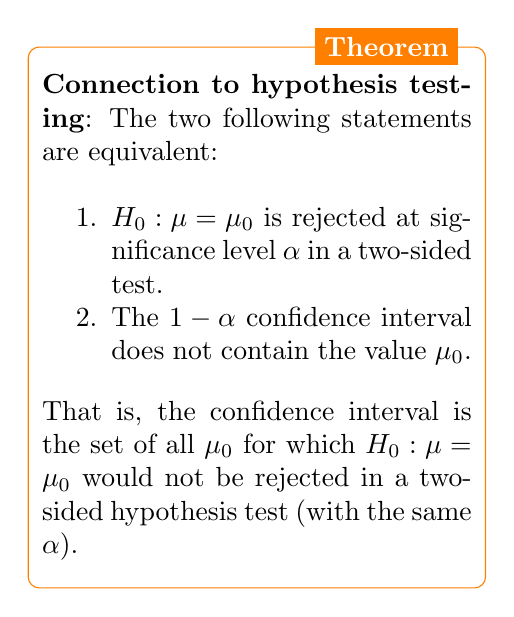
\begin{tikzpicture}
\node [rounded-box] (box){\begin{minipage}{0.45\textwidth}
    \textbf{Connection to hypothesis testing}: The two following statements are equivalent: \\

    \begin{enumerate}
        \item $H_0: \mu = \mu_0$ is rejected at significance level $\alpha$ in a two-sided test.
        \item The $1 - \alpha$ confidence interval does not contain the value $\mu_0$.
    \end{enumerate}

    \vspace{10pt}

    That is, the confidence interval is the set of all $\mu_0$ for which $H_0: \mu = \mu_0$ would not be rejected in a two-sided hypothesis test (with the same $\alpha$).
\end{minipage}};
\node[rounded-box-title, left=10pt] at (box.north east) {Theorem};
\end{tikzpicture}

\switchcolumn

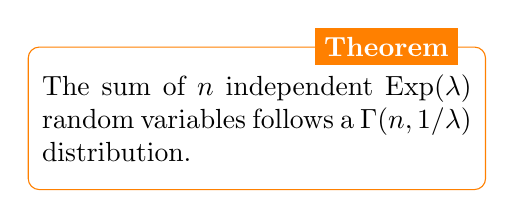
\begin{tikzpicture}
\node [rounded-box] (box){\begin{minipage}{0.45\textwidth}
    The sum of $n$ independent $\text{Exp}(\lambda)$ random variables follows a $\Gamma(n, 1 / \lambda)$ distribution.
\end{minipage}};
\node[rounded-box-title, left=10pt] at (box.north east) {Theorem};
\end{tikzpicture}

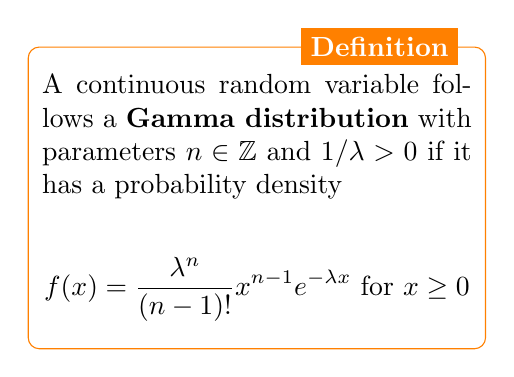
\begin{tikzpicture}
\node [rounded-box] (box){\begin{minipage}{0.45\textwidth}
    A continuous random variable follows a \textbf{Gamma distribution} with parameters $n \in \mathbb{Z}$ and $1 / \lambda > 0$ if it has a probability density
    
    $$f(x) = \frac{\lambda^n}{(n-1)!} x^{n-1} e^{-\lambda x} \text{ for } x \geq 0$$
\end{minipage}};
\node[rounded-box-title, left=10pt] at (box.north east) {Definition};
\end{tikzpicture}

\textbf{Problem}: The Gamma distribution depends on an \textbf{unknown parameter} $1 / \lambda$. Therefore, a random variable $S \sim \Gamma(n, 1 / \lambda)$ is not a pivot.

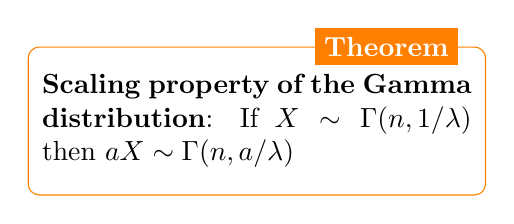
\begin{tikzpicture}
\node [rounded-box] (box){\begin{minipage}{0.45\textwidth}
    \textbf{Scaling property of the Gamma distribution}: If $X \sim \Gamma(n, 1 / \lambda)$ then $aX \sim \Gamma(n, a / \lambda)$
\end{minipage}};
\node[rounded-box-title, left=10pt] at (box.north east) {Theorem};
\end{tikzpicture}

(The Gamma scaling property follows from a similar scaling property of the Exponential distribution.)

\textbf{Solution}: $\lambda S \sim \Gamma(n, 1)$ is a pivot. Thus you can avoid the CLT approximation and instead use the known distribution.

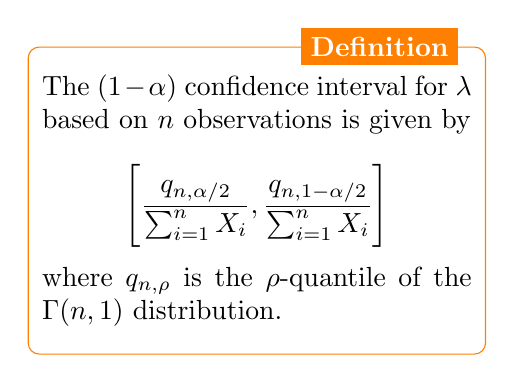
\begin{tikzpicture}
\node [rounded-box] (box){\begin{minipage}{0.45\textwidth}
    The $(1 - \alpha)$ confidence interval for $\lambda$ based on $n$ observations is given by

    $$\Bigg[ \frac{q_{n, \alpha / 2}}{\sum_{i=1}^n X_i}, \frac{q_{n, 1 - \alpha / 2}}{\sum_{i=1}^n X_i} \Bigg]$$

    where $q_{n, \rho}$ is the $\rho$-quantile of the $\Gamma(n, 1)$ distribution.
\end{minipage}};
\node[rounded-box-title, left=10pt] at (box.north east) {Definition};
\end{tikzpicture}

\textbf{Example}: Given a random variable $X \sim \text{Bin}(n, p)$, its test statistic is not a pivot because its distribution depends on an unknown parameter, $p$. By the CLT,

$$\frac{X - np}{\sqrt{np(1-p)}} \overset{d}{\rightarrow} \text{ as } n \rightarrow \infty \Rightarrow \frac{X - np}{\sqrt{np(1-p)}} \overset{d}{\approx} \mathcal{N}(0, 1)$$

Approximating $p$ by its sample estimate $\hat{p} = \frac{X}{n}$,

$$\frac{X - np}{\sqrt{n\hat{p}(1-\hat{p})}} \overset{d}{\rightarrow} \text{ as } n \rightarrow \infty \Rightarrow \frac{X - np}{\sqrt{n\hat{p}(1-\hat{p})}} \overset{d}{\approx} \mathcal{N}(0, 1)$$

This leads to the approximate confidence interval $\approx 1 - \alpha$, with $\hat{p} = X / n$, for $p$:

$$\Bigg[ \hat{p} - z_{\alpha / 2} \sqrt{\frac{\hat{p}(1-\hat{p})}{n}} , \hat{p} + z_{\alpha / 2} \sqrt{\frac{\hat{p}(1-\hat{p})}{n}} \Bigg] = \hat{p} \pm z_{\alpha / 2} \sqrt{\frac{\hat{p}(1-\hat{p})}{n}}$$

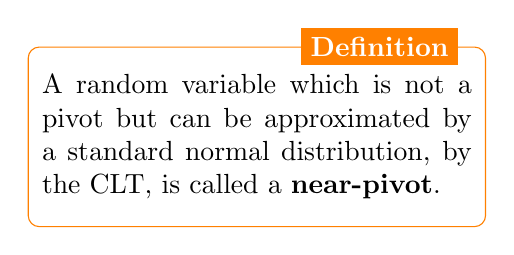
\begin{tikzpicture}
\node [rounded-box] (box){\begin{minipage}{0.45\textwidth}
    A random variable which is not a pivot but can be approximated by a standard normal distribution, by the CLT, is called a \textbf{near-pivot}.
\end{minipage}};
\node[rounded-box-title, left=10pt] at (box.north east) {Definition};
\end{tikzpicture}

\end{paracol}

\newpage

The critical value for a t-based confidence interval is always larger than the equivalent z-based critical value, because not only are we uncertain about the population mean, we are also uncertain about the population standard deviation. As sample size increases, $t$ converges to $z$.

\begin{verbatim}
# Suppose you are given a dataset that is sampled from a normally distributed population.
# The size of your dataset is 26, the sample mean is 23, and the sample standard deviation is 10.
# Compute the lower limit of the 80% confidence interval for mu.
sample_mean <- 23
sample_sd <- 10
sample_size <- 26
confidence_level <- 0.8
alpha <- 1 - confidence_level
critical_value <- qt(1 - alpha/2, df = sample_size - 1)
margin_of_error <- critical_value * (sample_sd / sqrt(sample_size))
lower_limit <- sample_mean - margin_of_error
print(lower_limit)

# Use R to generate a random sample of size 100 from a normal distribution with parameters mu=25, sigma=3.
# Compute the sample mean and standard deviation.
# Set the parameters
x <- rnorm(100, mean = 25, sd = 3)
sd(x)
mean(x)
t.test(x, mu = 25)
# If 1000 of your fellow MOOC students correctly solve this exercise, how many do you expect will answer "yes" on the previous subquestion?
# 950. There is a 95% probability of obtaining a random sample that gives rise to a confidence interval (computed with this technique) that does contain the actual value of mu.

set.seed(10)

# Run a simulation making one million 95% confidence intervals for the parameter lambda,
# based on samples of size 15 from an exponential distribution with parameter 0.923.
count1 <- 0
count2 <- 0
for (i in 1:1000000) {
  decays <- rexp(15, 0.923)
  CI_lower <- qgamma(0.025, 15, 1) / sum(decays)
  CI_upper <- qgamma(0.975, 15, 1) / sum(decays)
  if (CI_lower > 0.923) {
    count1 <- count1 + 1
  }
  if (CI_upper < 0.923) {
    count2 <- count2 + 1
  }
}
# What is the value of count1, the number of confidence intervals for which the
# lower bound is higher than the real value of the parameter?
count1
# How many intervals do contain the exact value of lambda?
count2
# Notice this means that ~95% of the confidence intervals contained the true parameter as expected.

\end{verbatim}
 \newpage
\section{Analysis of Variance (ANOVA)}

With ANOVA and the associated F test, one can examine the equality of multiple means using a single test:

$$H_0: \mu_1 = \mu_2 = \mu_3 = \dots, \quad H_A: \text{ At least one mean is different.}$$

Three conditions:
\begin{itemize}
    \item \textbf{Independence} of observations within and between groups.
    \item \textbf{Normality}, which can be investigated by checking if the group sizes are sufficiently large.
    \item \textbf{Constant variance} $\sigma^2$ in all groups ($\sigma^2$ may be known or unknown).
\end{itemize}

By default, we reject a null hypothesis when we get a p-value less than $\alpha = 0.05$.

The F statistic compares the between group variability (MSG) with the within group variability (MSE):

$$F = \frac{\text{MSG}}{\text{MSE}}$$

\begin{itemize}
    \item The MSG is the variance of $k$ means, so it has $k - 1$ degrees of freedom.
    \item The MSE is an average of $k$ individual group variances. It has $(n_1 - 1) + (n_2 - 1) + \dots = N - k$ degrees of freedom.
\end{itemize}

All else equal, the larger is $F$, the more inclined you should be to reject the null hypothesis.

If the null hypothesis is true, $F$ should be close to $1$ because the variability between groups with match the overall variability in the data.

If the null hypothesis is rejected (i.e. the F test indicates that at least one mean is different), one can proceed with multiple pairwise comparisons.

$$t = \frac{\bar{x}_1 - \bar{x}_2}{s \sqrt{\frac{1}{n_1} + \frac{1}{n_2}}}$$

\begin{itemize}
    \item It is good practice to use more stringent significance levels in pairwise comparisons to avoid making a Type I error.

    \item In addition, a pooled standard deviation should be used.

    \item \textbf{Bonferroni correction}: For a desired overall Type I error rate of $\alpha$, the Bonferroni correction suggests that a significance level $\alpha / K$ should be used for pairwise comparisons where $K$ is the number of pairwise comparisons.
\end{itemize}

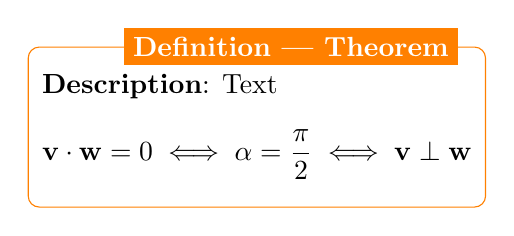
\begin{tikzpicture}
\node [rounded-box] (box){\begin{minipage}{0.45\textwidth}
    \textbf{Description}: Text
    $$\mathbf{v} \cdot \mathbf{w} = 0 \iff \alpha = \frac{\pi}{2} \iff \mathbf{v} \perp \mathbf{w}$$
\end{minipage}};
\node[rounded-box-title, left=10pt] at (box.north east) {Definition | Theorem};
\end{tikzpicture}
 \newpage
\section{Analysis of Categorical Data}

\begin{paracol}{2}

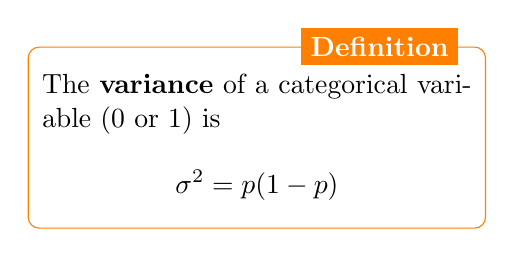
\begin{tikzpicture}
\node [rounded-box] (box){\begin{minipage}{0.45\textwidth}
    The \textbf{variance} of a categorical variable ($0$ or $1$) is

    $$\sigma^2 = p (1-p)$$
\end{minipage}};
\node[rounded-box-title, left=10pt] at (box.north east) {Definition};
\end{tikzpicture}

\textbf{Proof}: Recall the variance is defined as the average squared deviation from the mean. For $1$, the squared deviation from the mean is $(1-p)^2$; for $0$, it is $p^2$.

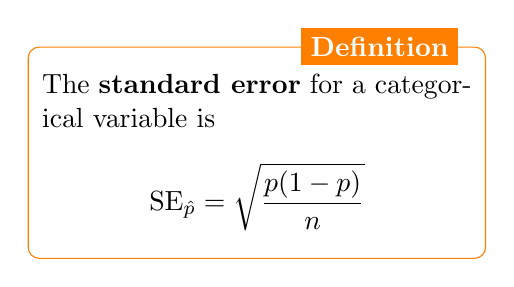
\begin{tikzpicture}
\node [rounded-box] (box){\begin{minipage}{0.45\textwidth}
    The \textbf{standard error} for a categorical variable is

    $$\text{SE}_{\hat{p}} = \sqrt{\frac{p(1-p)}{n}}$$
\end{minipage}};
\node[rounded-box-title, left=10pt] at (box.north east) {Definition};
\end{tikzpicture}

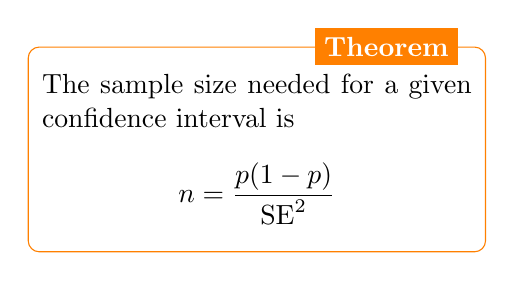
\begin{tikzpicture}
\node [rounded-box] (box){\begin{minipage}{0.45\textwidth}
    The sample size needed for a given confidence interval is

    $$n = \frac{p(1-p)}{\text{SE}^2}$$
\end{minipage}};
\node[rounded-box-title, left=10pt] at (box.north east) {Theorem};
\end{tikzpicture}

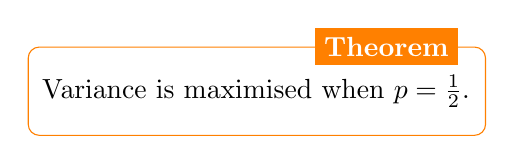
\begin{tikzpicture}
\node [rounded-box] (box){\begin{minipage}{0.45\textwidth}
    Variance is maximised when $p = \frac{1}{2}$.
\end{minipage}};
\node[rounded-box-title, left=10pt] at (box.north east) {Theorem};
\end{tikzpicture}

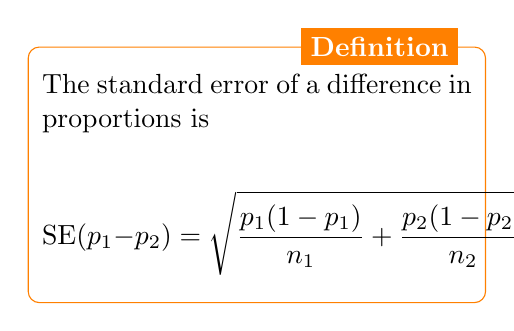
\begin{tikzpicture}
\node [rounded-box] (box){\begin{minipage}{0.45\textwidth}
    The standard error of a difference in proportions is

    $$\text{SE}(p_1 - p_2) = \sqrt{\frac{p_1(1-p_1)}{n_1} + \frac{p_2(1-p_2)}{n_2}}$$
\end{minipage}};
\node[rounded-box-title, left=10pt] at (box.north east) {Definition};
\end{tikzpicture}

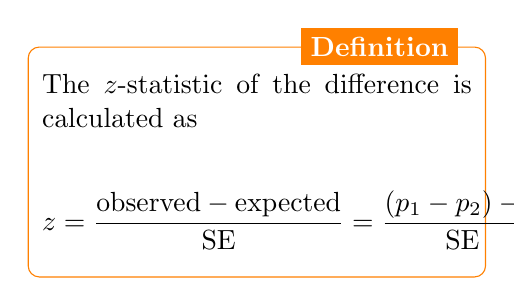
\begin{tikzpicture}
\node [rounded-box] (box){\begin{minipage}{0.45\textwidth}
    The $z$-statistic of the difference is calculated as

    $$z = \frac{\text{observed} - \text{expected}}{\text{SE}} = \frac{(p_1 - p_2) - 0}{\text{SE}}$$
\end{minipage}};
\node[rounded-box-title, left=10pt] at (box.north east) {Definition};
\end{tikzpicture}

\switchcolumn

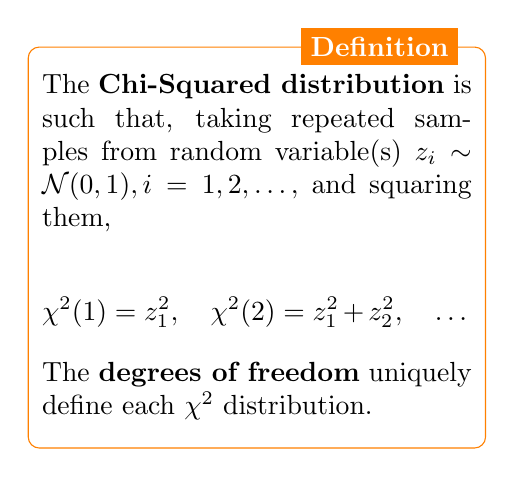
\begin{tikzpicture}
\node [rounded-box] (box){\begin{minipage}{0.45\textwidth}
    The \textbf{Chi-Squared distribution} is such that, taking repeated samples from random variable(s) $z_i \sim \mathcal{N}(0, 1), i = 1, 2, \dots,$ and squaring them,

    $$\chi^2(1) = z_1^2, \quad \chi^2(2) = z_1^2 + z_2^2, \quad \dots$$

    The \textbf{degrees of freedom} uniquely define each $\chi^2$ distribution.
\end{minipage}};
\node[rounded-box-title, left=10pt] at (box.north east) {Definition};
\end{tikzpicture}

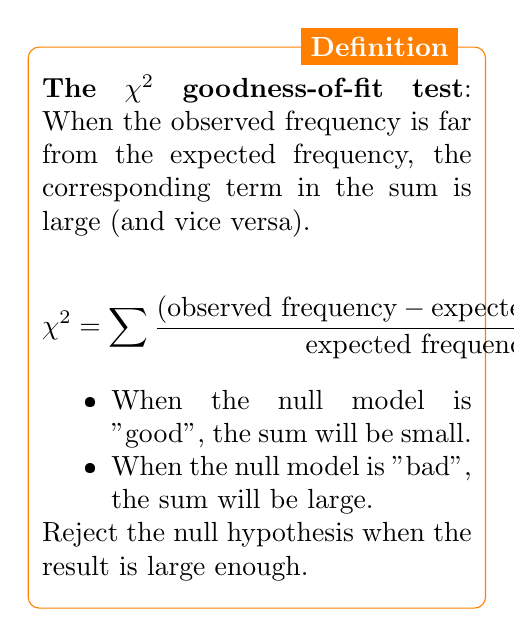
\begin{tikzpicture}
\node [rounded-box] (box){\begin{minipage}{0.45\textwidth}
    \textbf{The $\chi^2$ goodness-of-fit test}: When the observed frequency is far from the expected frequency, the corresponding term in the sum is large (and vice versa).

    $$\chi^2 = \sum \frac{(\text{observed frequency} - \text{expected frequency})^2}{\text{expected frequency}}$$

    \begin{itemize}
        \item When the null model is "good", the sum will be small.
        \item When the null model is "bad", the sum will be large.
    \end{itemize}

    Reject the null hypothesis when the result is large enough.
\end{minipage}};
\node[rounded-box-title, left=10pt] at (box.north east) {Definition};
\end{tikzpicture}

\textbf{Example}:

\begin{align*}
    \chi^2 & = \frac{(4-10)^2}{10} + \frac{(6-10)^2}{10} + \frac{(17-10)^2}{10} \\
    & = \frac{6^2}{10} + \frac{4^2}{10} + \frac{7^2}{10} \\
    & = 10.1
\end{align*}

Reject the null hypothesis when the result of the $\chi^2$ test is large enough - compare with the appropriate $\chi^2$ distribution with $k-1$ degrees of freedom.

\end{paracol}
 \newpage
\section{Linear Regression}

\begin{paracol}{2}

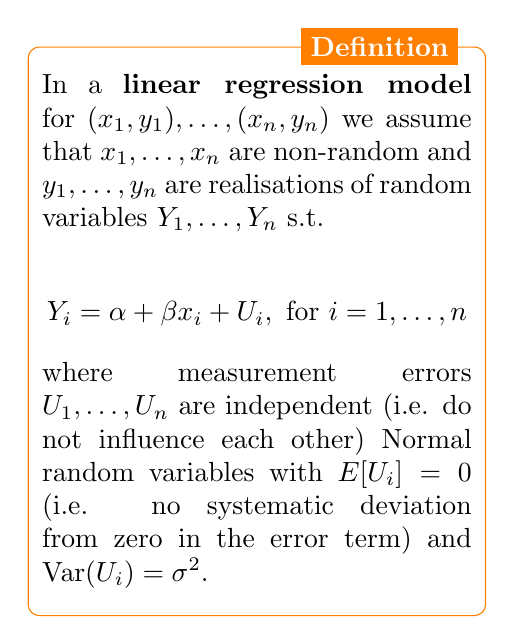
\begin{tikzpicture}
\node [rounded-box] (box){\begin{minipage}{0.45\textwidth}
    In a \textbf{linear regression model} for $(x_1, y_1), \dots, (x_n, y_n)$ we assume that $x_1, \dots, x_n$ are non-random and $y_1, \dots, y_n$ are realisations of random variables $Y_1, \dots, Y_n$ s.t.

    $$Y_i = \alpha + \beta x_i + U_i, \text{ for } i = 1, \dots, n$$

    where measurement errors $U_1, \dots, U_n$ are independent (i.e. do not influence each other) Normal random variables with $E[U_i] = 0$ (i.e. no systematic deviation from zero in the error term) and $\text{Var}(U_i) = \sigma^2$.
\end{minipage}};
\node[rounded-box-title, left=10pt] at (box.north east) {Definition};
\end{tikzpicture}

\switchcolumn

\begin{tikzpicture}
\node [rounded-box] (box){\begin{minipage}{0.45\textwidth}
    The least squares estimators $\hat{\alpha}, \hat{\beta}$ that minimise the sum of squared distances

    $$\sum_{i=1}^n (y_i - \alpha - \beta x_i)^2$$

    over all $\alpha, \beta \in \mathbb{R}$ are given by

    $$\hat{\alpha} = \bar{Y}_n - \hat{\beta} \bar{x}_n$$
    $$\hat{\beta} = \frac{\sum_{i=1}^n (x_i - \bar{x}_n)(Y_i - \bar{Y}_n)}{\sum_{i=1}^n (x_i - \bar{x}_n)^2} = \frac{s_Y}{s_X}r_{x,Y}$$

    which are both unbiased; that is, $E[\hat{\alpha}] = \alpha, E[\hat{\beta}] = \beta$.

    Since, according to the model, $U_i = Y_i - \alpha - \beta x_i \approx Y_i - \hat{\alpha} - \hat{\beta} x_i$, the least squares estimator for $\sigma^2$ is given by

    $$\hat{\sigma^2} = \frac{1}{n-2} \sum_{i=1}^n (Y_i - \hat{\alpha} - \hat{\beta} x_i)^2$$

    where dividing by $n-2$ gives an unbiased estimator, given the expression contains two estimated parameters $\hat{\alpha}, \hat{\beta}$.
\end{minipage}};
\node[rounded-box-title, left=10pt] at (box.north east) {Theorem};
\end{tikzpicture}

\switchcolumn

\begin{tikzpicture}
\node [rounded-box] (box){\begin{minipage}{0.45\textwidth}
    If $U_1, \dots, U_n \sim \mathcal{N}(0, \sigma^2)$, the least squares estimators $\hat{\alpha}, \hat{\beta}$ obtained with the method of moments are the same as the maximum likelihood estimators $\hat{\alpha}_{ML}, \hat{\beta}_{ML}$.
\end{minipage}};
\node[rounded-box-title, left=10pt] at (box.north east) {Theorem};
\end{tikzpicture}

\end{paracol}

\subsection{Model Assessment}

\begin{paracol}{2}

\begin{tikzpicture}
\node [rounded-box] (box){\begin{minipage}{0.45\textwidth}
    Let $\hat{\alpha}, \hat{\beta}$ be the least-squares estimators. Then for each observation, the $i$-\textbf{residual} is the observed minus predicted:

    $$R_i = Y_i - \hat{\alpha} - \hat{\beta} x_i, i = 1, 2, \dots, n$$
\end{minipage}};
\node[rounded-box-title, left=10pt] at (box.north east) {Definition};
\end{tikzpicture}

Since $\hat{\alpha}, \hat{\beta}$ are unbiased estimators, i.e. $E[\hat{\alpha}] = \alpha, E[\hat{\beta}] = \beta$, the residuals $R_i = Y_i - \hat{\alpha} - \hat{\beta} x_i$ mimic the unobservable measurement errors $U_i = Y_i - \alpha - \beta x_i$:

\vspace{-10pt}

$$R_i \approx U_i$$

A \textit{residual plot} can be used to check the model \textbf{assumptions}:

\begin{itemize}
    \item Linearity: Is there a linear relationship?
    \item Is $E[U_i] = 0$?
    \item \textbf{Homoskedasticity}: Is $\text{Var}(U_i) = \sigma^2$? That is, is the variation of the residuals constant along the line?
    \item Nearly-normal residuals: Is $U_i \sim \mathcal{N}(0, \sigma^2)$? (straight line in QQ-Plot)
\end{itemize}

\begin{tikzpicture}
\node [rounded-box] (box){\begin{minipage}{0.45\textwidth}
    The variation in $Y$ is defined as the \textbf{total sum of squares}

    $$\text{SS}_{\text{tot}} = \sum_{i=1}^n (y_i - \bar{y}_n)^2$$

    The variation in $Y$ due to measurement error is quantified by the \textbf{residual sum of squares}

    $$\text{SS}_{\text{res}} = \sum_{i=1}^n R_i^2$$
\end{minipage}};
\node[rounded-box-title, left=10pt] at (box.north east) {Definition};
\end{tikzpicture}

\switchcolumn

The remaining variation in $Y$ is due to the linear relationship with $x$, and the higher its share of the total variation the better the fit of the model:

\begin{tikzpicture}
\node [rounded-box] (box){\begin{minipage}{0.45\textwidth}
    Let $\text{SS}_\text{tot}, \text{SS}_\text{res}$ be the total sum of squares and the residual sum of squares. Then the \textbf{proportion of explained variance} is the \textbf{coefficient of determination}

    $$R^2 = 1 - \frac{\text{SS}_\text{tot}}{\text{SS}_\text{res}} (= r_{x, Y}^2)$$

    (which is equal to the squared correlation coefficient between $x$ and $Y$).
\end{minipage}};
\node[rounded-box-title, left=10pt] at (box.north east) {Definition};
\end{tikzpicture}

The least squares estimate $\hat{\sigma}^2 = \frac{1}{n-2} \sum_{i=1}^n R_i^2$, by definition.

\begin{tikzpicture}
\node [rounded-box] (box){\begin{minipage}{0.45\textwidth}
    The \textbf{standard error} is defined as

    $$\text{SE} = \sqrt{\frac{1}{n-2} \sum_{i=1}^n R_i^2}$$
\end{minipage}};
\node[rounded-box-title, left=10pt] at (box.north east) {Definition};
\end{tikzpicture}

\end{paracol}

\newpage

\subsection{Tests and Confidence Intervals}

\begin{paracol}{2}

\begin{tikzpicture}
\node [rounded-box] (box){\begin{minipage}{0.45\textwidth}
    Consider the simple linear regression model $Y_i = \alpha + \beta x_i + U_i, i = 1, 2, \dots, n$ with i.i.d. $U_i, U_2, \dots, U_n \sim \mathcal{N}(0, \sigma^2)$. Let $\hat{\alpha}, \hat{\beta}$ be the least squares estimators. Then

    $$\frac{\hat{\alpha} - \alpha}{\text{se}(\hat{\alpha})}, \frac{\hat{\beta} - \beta}{\text{se}(\hat{\beta})} \sim t(n-2)$$

    follow a $t$-distribution with $m = n-2$ degrees of freedom.
\end{minipage}};
\node[rounded-box-title, left=10pt] at (box.north east) {Theorem};
\end{tikzpicture}

\switchcolumn

Thus, confidence intervals can be constructed for the least squares estimators:

$$P \Bigg( -t_{n-1, \alpha / 2} \leq \frac{\hat{\beta} - \beta}{\text{se}(\hat{\beta})} \leq t_{n-2, \alpha / 2} \Bigg) = 1 - \alpha$$

$$P \Bigg( \hat{\beta} - t_{n-1, \alpha / 2} \text{se}(\hat{\beta}) \leq \beta \leq \hat{\beta} + t_{n-1, \alpha / 2} \text{se}(\hat{\beta}) \Bigg) = 1 - \alpha$$

\end{paracol}

Note: With just one $x$-variable the $t$-test for $\beta$ is equivalent to what is called the F-test. Both testing problems are different with multiple $x$-variables in a multiple linear regression model.

\subsection{Model Selection}

\begin{paracol}{2}

Potential fixes if model assumptions are not satisfied:

\begin{itemize}
    \item A quadratic term is a potential fix for a parabola in the residual plot (and should result in a straight line).
    \item Log-scaling the independent variable is a potential fix for heteroskedasticity (and should result in constant variance in the residual plot, i.e. homoskedasticity).
\end{itemize}

\quad

Products of variables are called \textbf{interaction terms}.

\switchcolumn

\begin{tikzpicture}
\node [rounded-box] (box){\begin{minipage}{0.45\textwidth}
    The \textbf{Akaike Information Criterion (AIC)} is a measure of the suitability of the dependent variables in a model:

    $$AIC = 2k - 2 \log(L)$$

    where $k$ is the number of dependent variables, and $L$ is the likelihood. Both terms increase with the number dependent variables. \\
    
    Therefore, you want the AIC to be as low as possible.
\end{minipage}};
\node[rounded-box-title, left=10pt] at (box.north east) {Definition};
\end{tikzpicture}

\end{paracol}
 \newpage
\section{Generalised Linear Models (GLMs)}

Generalisations of the linear model include:

\begin{itemize}
	\item Classification problems: logistic regression, support vector machines
	\item Non-linearity: kernel smoothing, splines and generalised additive models, nearest neighbour methods
	\item Interactions: tree-based methods, bagging, random forests and boosting
	\item Regularised fitting: Ridge and Lasso
\end{itemize}

\begin{tikzpicture}
	\node [rounded-box] (box){\begin{minipage}{0.975\textwidth}
			A $n^\text{th}$-order spline with knots at $\xi_k, k = 1, \dots, K$ is a piecewise $n^\text{th}$-order polynomial with continuous derivatives up to order $n-1$ at each knot.

			$$y_i = \beta_0 + \beta_1 b_1(x_i) + \beta_2 b_2(x_i) + \dots + \beta_{K+n} b_{K+n}(x_i) + \epsilon_i$$

			$$b_1(x_i) = x_i, \quad b_2(x_i) = x_i^2, \quad \dots, \quad b_{k+n}(x_i) = (x_i - \xi_k)^n_+, \quad k = 1, \dots, K$$

			$$(x_i - \xi_k)^n_+ = \begin{cases}
					(x_i - \xi_k)^3 & \text{if } x_i > \xi_k \\
					0               & \text{otherwise}
				\end{cases}$$
		\end{minipage}};
	\node[rounded-box-title, left=10pt] at (box.north east) {Definition};
\end{tikzpicture}

A cubic spline with $K$ knots has $K + 4$ parameters, or degrees of freedom. A \textbf{natural spline} with $K$ knots has $K$ degrees of freedom.

A natural cubic spline extrapolates linearly beyond the boundary knots. This adds $4 = 2 \times 2$ extra constraints, and allows us to put more internal knots for the same degrees of freedom as a regular cubic spline.

\textbf{Smoothing splines} avoid the knot-selection issue, leaving a single $\lambda$ to be chosen. Consider this criterion for fitting a smooth function $g(x)$ to some data:

$$\min_{g \in S} \sum_{i=1}^n (y_i - g(x_i))^2 + \lambda \int g''(t)^2 \, dt$$

\begin{itemize}
	\item The first term is the RSS, and tries to make $g(x)$ match the data at each $x_i$.
	\item The second term is a rougness penalty, and controls how wiggly $g(x)$ is. It is modulated by the tuning parameter $\lambda \geq 0$.
	      \begin{itemize}
		      \item The smaller $\lambda$, the more wiggly the function, eventually interpolating $y_i$ when $\lambda = 0$.
		      \item As $\lambda \rightarrow \infty$, the function $g(x)$ becomes linear.
	      \end{itemize}
\end{itemize}

The solution is a natural cubic spline with a knot at every unique value of $x_i$. The roughness penalty still controls the roughness via $\lambda$.

\begin{tikzpicture}
	\node [rounded-box] (box){\begin{minipage}{0.45\textwidth}
			\textbf{Description}: Text
			$$\mathbf{v} \cdot \mathbf{w} = 0 \iff \alpha = \frac{\pi}{2} \iff \mathbf{v} \perp \mathbf{w}$$
		\end{minipage}};
	\node[rounded-box-title, left=10pt] at (box.north east) {Definition | Theorem};
\end{tikzpicture}
 \newpage

\nocite{*}
\printbibliography

\end{document}
